%%%%%%%%%%%%%%%%%%%%%%%%%%%%%%%%%%%%%%%%%%%%%%%%%%%%%%%%%%%%%%%%%%% 
%                                                                 %
%                            CHAPTER SEVEN                         %
%                                                                 %
%%%%%%%%%%%%%%%%%%%%%%%%%%%%%%%%%%%%%%%%%%%%%%%%%%%%%%%%%%%%%%%%%%% 
 
\chapter{AERODYNAMIC SHAPE OPTIMIZATION}
The last application is a single-point Euler-based aerodynamic shape optimization problem on the NASA Common Research Model (CRM) wing~\cite{crm_wing} defined by the Aerodynamic Design Optimization Discussion Group (ADODG) ~\cite{adodg}, in which the drag coefficient is minimized with lift, pitching moment, and geometric constraints.    Previously, Lyu et al. presented a comprehensive set of results on aerodynamic shape optimization of the NASA CRM wing based on a RANS model with large numbers of shape variables using SNOPT~\cite{2015lyu_crm}. Although the study in this thesis at this stage is based on the Euler model and a coarser mesh grid than those in~\cite{2015lyu_crm}, the long term objective is to run on RANS model with a fine mesh.   

\section{Problem Description}
The baseline wing-only geometry is extracted from the CRM wing-body configuration with a blunt trailing edge. An IGES file is provided to the public as shown in Figure~\ref{fig:crm_wing}. The CRM is of a contemporary transonic commercial airline, with a size similar to that of Boeing 777. It has been optimized in aerodynamic performance, but with an aggressive pressure recovery in the outboard wing to be researched on, to provide room for performance improvements. 
The nominal cruise flight condition for Boeing 777 is at Mach 0.85 and a Reynolds number of 5 million based on the mean aerodynamic chord. 

The following geometric information are already given by ADODG, 
The origin of the coordinate system is at the leading edge of the wing root, and all coordinates are scaled by the mean aerodynamic chord of 275.8 inches. Pitching moments are measured about the point $(1.2077, 0, 0.007669)$ using the reference length in units. All aerodynamic coefficients are computed in reference to the projected area $S_{\text{ref}}=3.407014$ squared reference units. 

\begin{figure}[tbp]
  \centering
  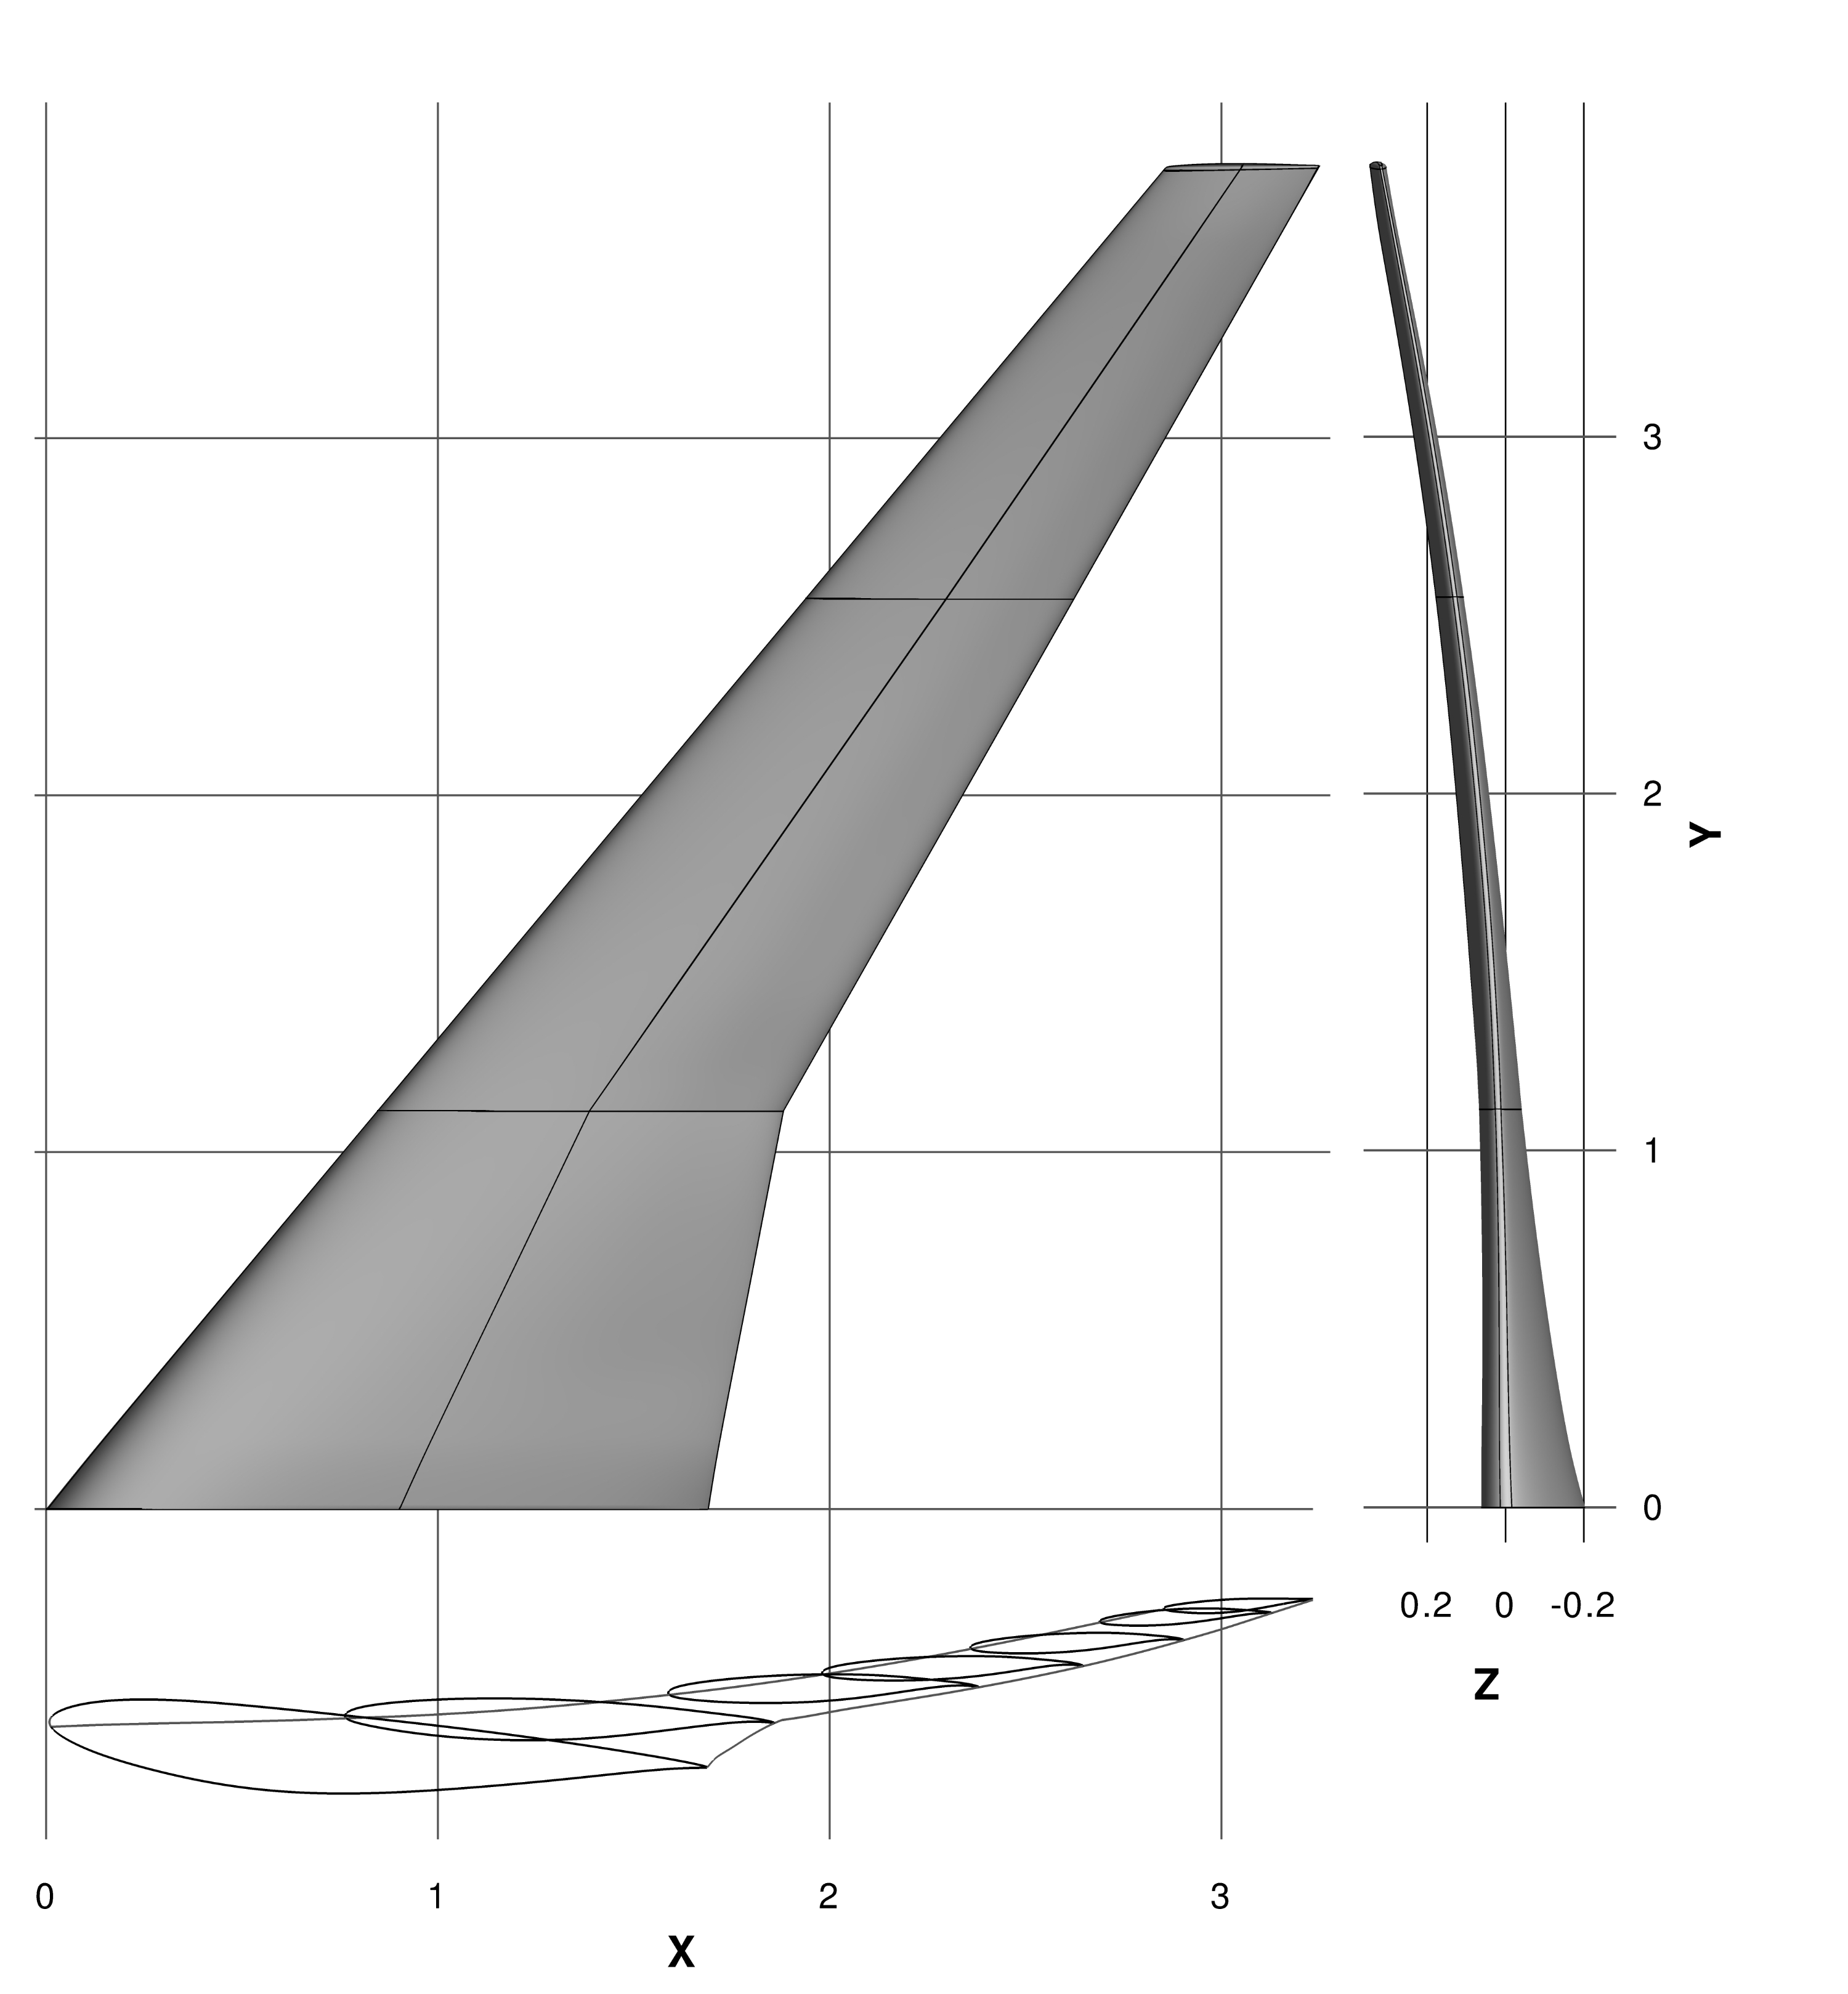
\includegraphics[clip,width=0.75\textwidth]{./figs/chap7_aso/CRM-wing.png}%
  \caption{CRM wing \label{fig:crm_wing}}
\end{figure}


\subsection{Mesh Generation, Parameterization and Flow Solver}
The mesh CGNS file is generated by Michigan MDOLab's in-house hyperbolic mesh generator using an O-grid topology method from the wing surface to a garfield 25 times of the wing span. Three levels of mesh are available for Euler cases as shown in Table~\ref{tab:euler_mesh}:

\begin{table}[H]
  \begin{center}
    \caption{Three grid levels and baseline aerodynamic coefficients for the Euler cases
    \label{tab:euler_mesh}}
  \begin{tabular}{ c r c c c c }
 \textbf{Mesh level}   &  \textbf{Mesh size}  & \textbf{CD} & \textbf{CL}  & \textbf{CM} & $\mathbf{\alpha}$  \\\hline
 L0                  &  840,192   & 0.00995   & 0.49879 & -0.20182  & $2.5^{\circ}$   \\
 L1                  &  105,024   & 0.01085   & 0.48925 & -0.19502    & $2.5^{\circ}$ \\
 L2 		      &   13,000    &  0.01417   & 0.46638    & -0.18142  &  	$2.5^{\circ}$ 	 
  \end{tabular}
  \end{center}
\end{table}

The wing geometry is parameterized using a free-form deformation (FFD) volume method~\cite{Kenway:2010:C}, where the wing geometry is embedded inside a FFD box, and the geometric changes of the wing surface are performed by changing the outer shape of the FFD volume. The derivatives of the wing surface points to the design variables representing the changes to the outer boundary of the FFD are easily available since FFD uses B-spline volumes. Figure~\ref{fig:crm_ffd} shows the FFD volume and the control points, where the displacement of the control points in the vertical (z) direction are the design variables. 

 \begin{figure}[tbp]
  \centering
  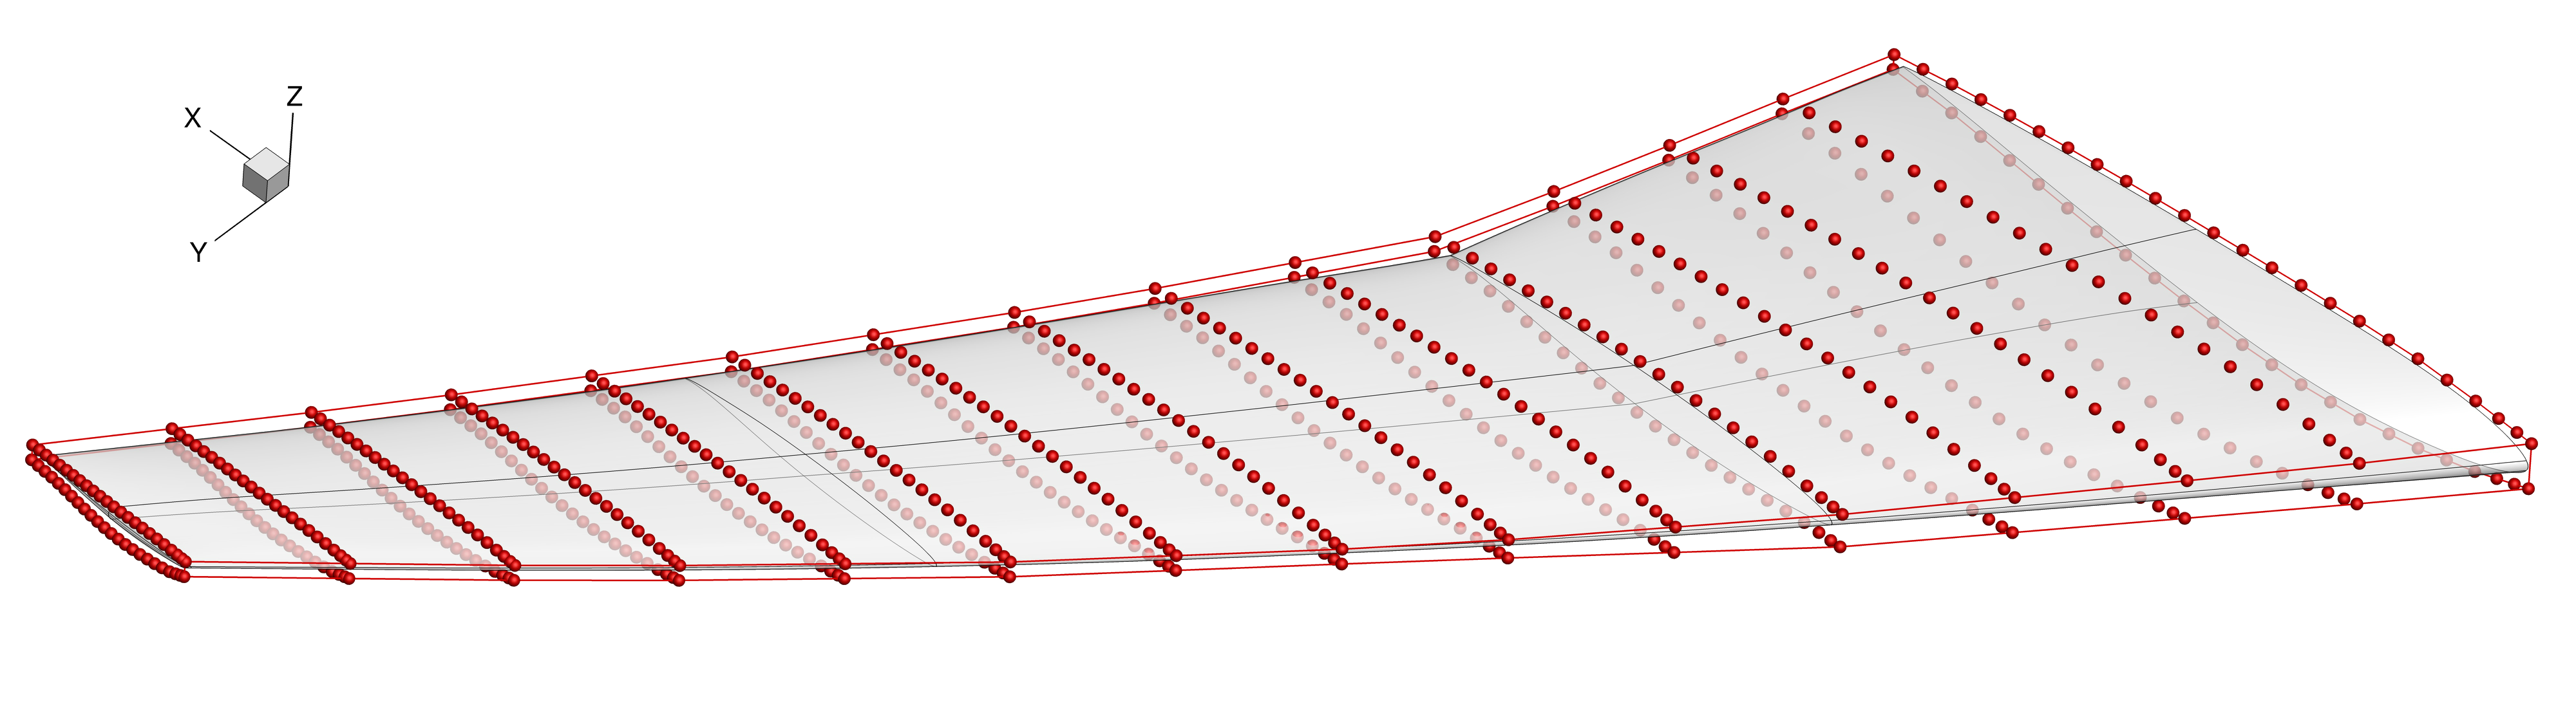
\includegraphics[clip,width=0.8\textwidth]{./figs/chap7_aso/CRM-wing-FFD.png}%
  \caption{CRM FFD \label{fig:crm_ffd}}
\end{figure}

The flow solver used in this study is SUmb~\cite{sumb_pdf}, a finite-volume, cell-centered multi-block structured general flow solver that can solve a variety type of problems, including the compressible Euler, laminar Navier-Stokes and Reynolds-Averaged Navier-Stokes (RANS) equations. In this study, the compressible Euler equations are used. The DRP cluster on Rensselaer Polytechnic Institute's CCI is used, consisting of 64 nodes, and each node has 128GB of system memory and two eight-core 2.6 GHz Intel Xeon E5-2650 processors. 

\subsection{Optimization Formulation}
When doing optimization, sectional shapes are allowed to change by changing the vertical (z) coordinates 
of each pair of top and bottom surface points in $n_x$ chord wise locations across the $n_y$ spanwise sections. The leading and trailing edges of the root section are fixed. For the other sections, the trailing edge are fixed while the leading edge is free. This way arbitrary wing twists could be implicitly represented by the remaining degrees of freedom. The wing planform is fixed, and the angle of attack is permitted to change.  

The optimization problem can be formulated as: 
\begin{equation*}
  \begin{alignedat}{2}
    \underset{x, \alpha}{\text{min}} \quad & C_D && \alpha: \text{angle of attack}; x:\text{FFD control points}   \\
    \text{subject to} \quad & C_L \geq 0.5  && \text{Lift coefficient constraint}   \\
      & C_{M_y} \geq -0.17          && \text{Pitching moment constraint}   \\
      & t \geq 0.25 t_{\text{base}} && \text{Minimum thickness constraints}   \\
      & V \geq V_{\text{base}} && \text{Minimum volume constraint}   \\
      & \Delta z_{TE, \text{upper}} = -\Delta z_{TE, \text{lower}}  && \text{Fixed trailing edge constraints}   \\
      & \Delta z_{LE, \text{upper, root}} = -\Delta z_{LE, \text{lower, root}} && \text{Fixed leading edge of the wing root}  
  \end{alignedat}
\end{equation*}
The thicknesss constraints are imposed in 25 chord wise locations from 1\% to 99\% local chord and 30 span wise locations covering the full span.  The number of design variables include the angle of attack plus the shape design variables, or the number of FFD control points. The distributions of the FFD control points are listed in Table~\ref{tab:ffd_sizes}. Each spanwise station indicate a distinct airfoil shape, and the chordwise points control the shape of each airfoil, with half on the top and half on the bottom.  
 
\begin{table}[tbp]
  \begin{center}
    \caption{Number of design variables from six different FFD boxes
    \label{tab:ffd_sizes}}
  \begin{tabular}{ l c c c c c c}
         & $\mathbf{72}$  & $\mathbf{192}$ & $\mathbf{320}$
    & $\mathbf{480}$  &  $\mathbf{616}$  &  $\mathbf{768}$   \\
    \hline
    % \rule{0ex}{3ex}%
    Chordwise  &   6 & 12  & 16  & 20 & 22 & 24 \\ 
    Spanwise &   6 & 8 & 10  & 12 & 14 & 16 \\  
    Vertical  &   2 & 2 & 2 & 2  & 2 & 2
  \end{tabular}
  \end{center}
\end{table}

The lift coefficient $C_L$, drag coefficient $C_D$ and pitching moment coefficient $C_{M_y}$ are aerodynamic coefficients calculated from the state variables - fluid mass density, velocity and pressure distributions across the mesh domain. While the state variables are related with the wing surface shape through the compressible Euler equations.  The flight condition considered is at Mach number 0.65. 


\section{Results}
This section presents the convergence results for both Kona and SNOPT. For Kona, the convergence plots contain 
the iteration history of the infinity norm of the Complementarity products, the feasibility and optimality. For SNOPT, 
the history of the merit function, the feasibility and optimality are plotted. Note that the definition of feasibility and optimality in Kona and SNOPT are slightly different. So it is reasonable that the two doesn't match each other exactly. 
However, we can still get a conceptual idea of the progress of the optimization.    
\subsection{Results-Kona}
Figure~\ref{fig:kona_192}, \ref{fig:kona_480}, and \ref{fig:kona_768} shows the plots for the L1 grid, with no. of 
design variables ranges from 192, 480 to 768. The first subplot in those figures shows the complementarity, feasibility and optimality history, while the second subplots shows history $CD$, $CL$, and $CMy$. Note that the 
optimality and feasibility are only reduced by approximately $10^{-2}$, but that is also the case for SNOPT as shown in the figures in the next subsection. In addition, Figure 7 in~\cite{2015lyu_crm} also exhibits similar amount of 
reduction in feasibility and optimality, although Figure 7 in~\cite{2015lyu_crm} is for RANS case. 

Note that in Kona, the $CD$, $CL$, and $CMy$ do not conform to the inequality constraints very quickly, and they 
stay a little far from it for the first half of the iteration. That could be explained by the stronger influence of the homotopy term on the optimization steps. At the second half, the inequality constraints are satisfied.   

\begin{figure}[H]
  \centering
   \subfloat[\label{fig:kona192opt}]{
   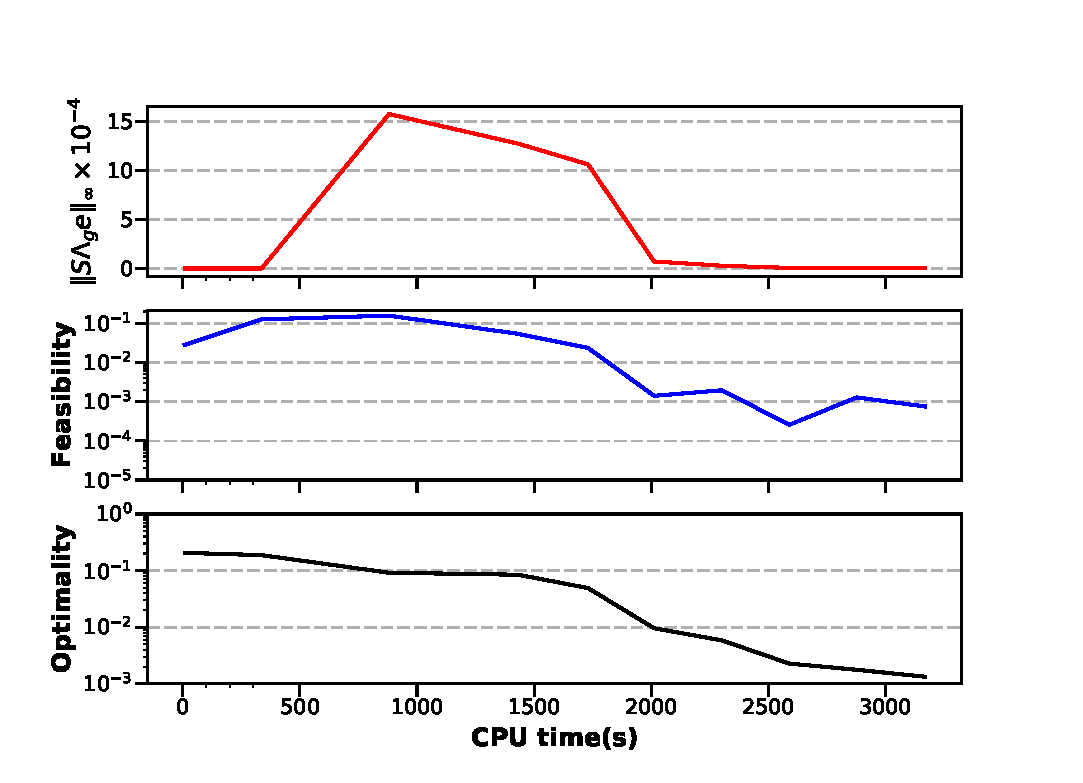
\includegraphics[clip,width=0.55\textwidth]{./figs/chap7_aso/kona/L1_192_comp_opt_feas.eps} } 
  % \hspace{1em}
  \subfloat[\label{fig:kona192cd}]{
   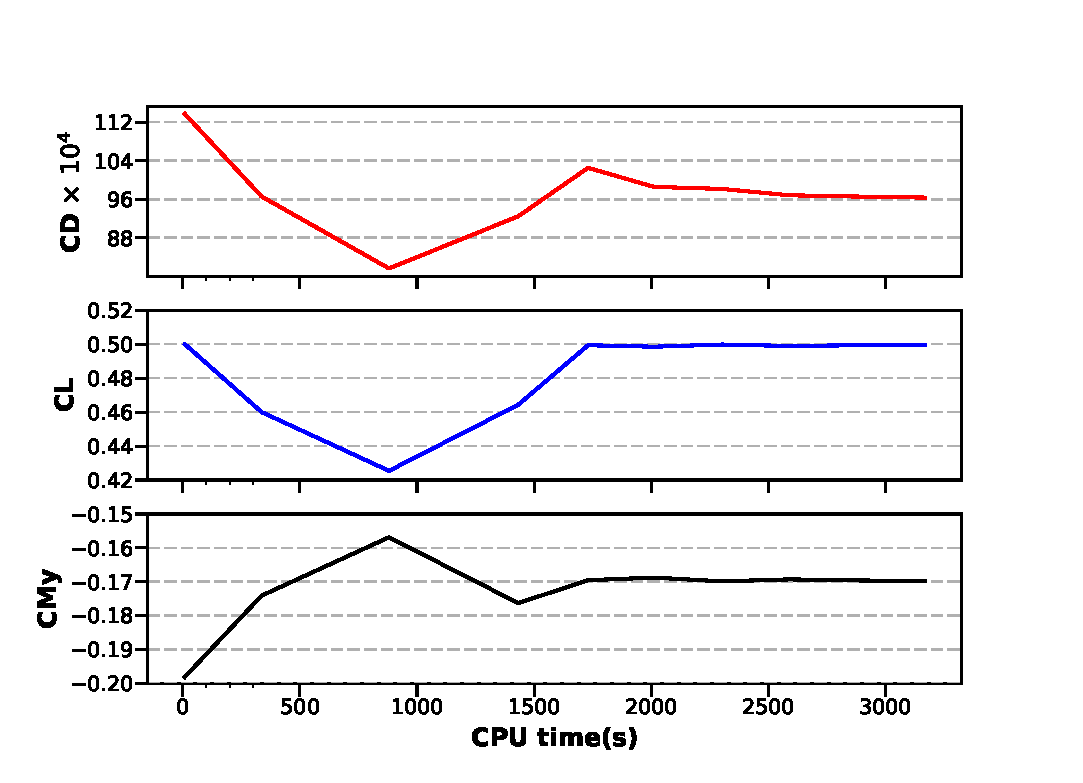
\includegraphics[clip,width=0.55\textwidth]{./figs/chap7_aso/kona/L1_192_cdlm.eps} }
  % \hspace{1em}
   \caption{Convergence histories for L1 grid, no. of design 192 \label{fig:kona_192}}
\end{figure}

\begin{figure}[H]
  \centering
   \subfloat[\label{fig:kona480opt}]{
   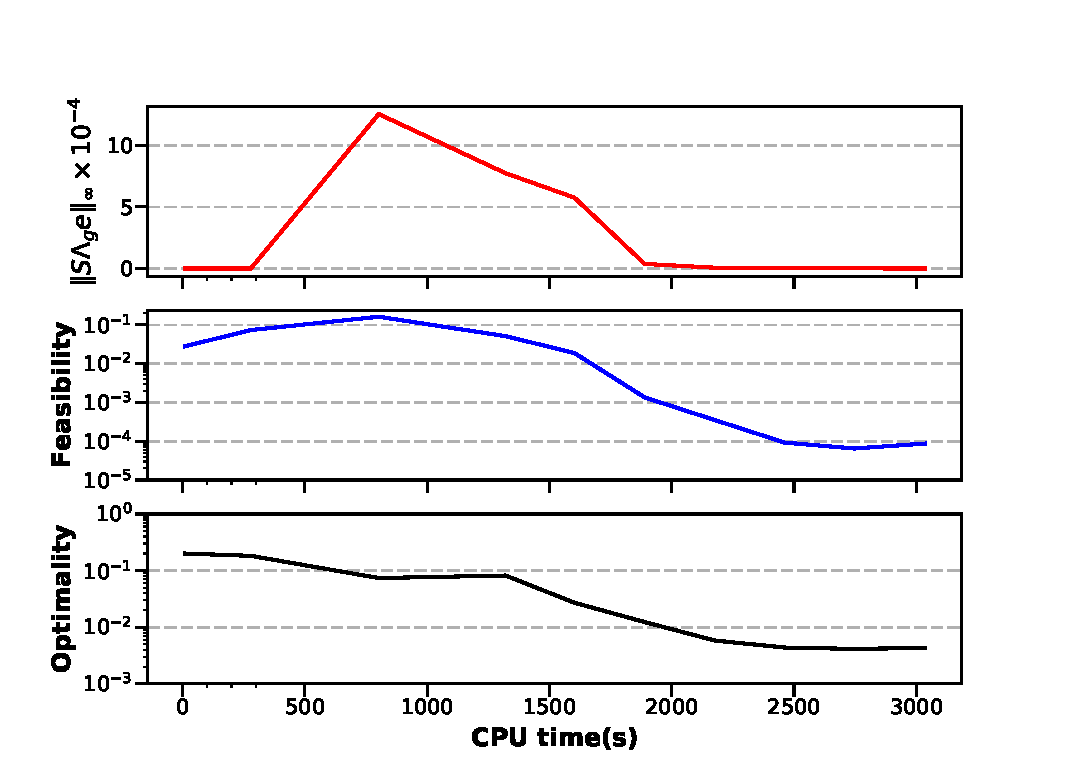
\includegraphics[clip,width=0.55\textwidth]{./figs/chap7_aso/kona/L1_480_comp_opt_feas.eps} } 
  % \hspace{1em}
  \subfloat[\label{fig:kona480cd}]{
   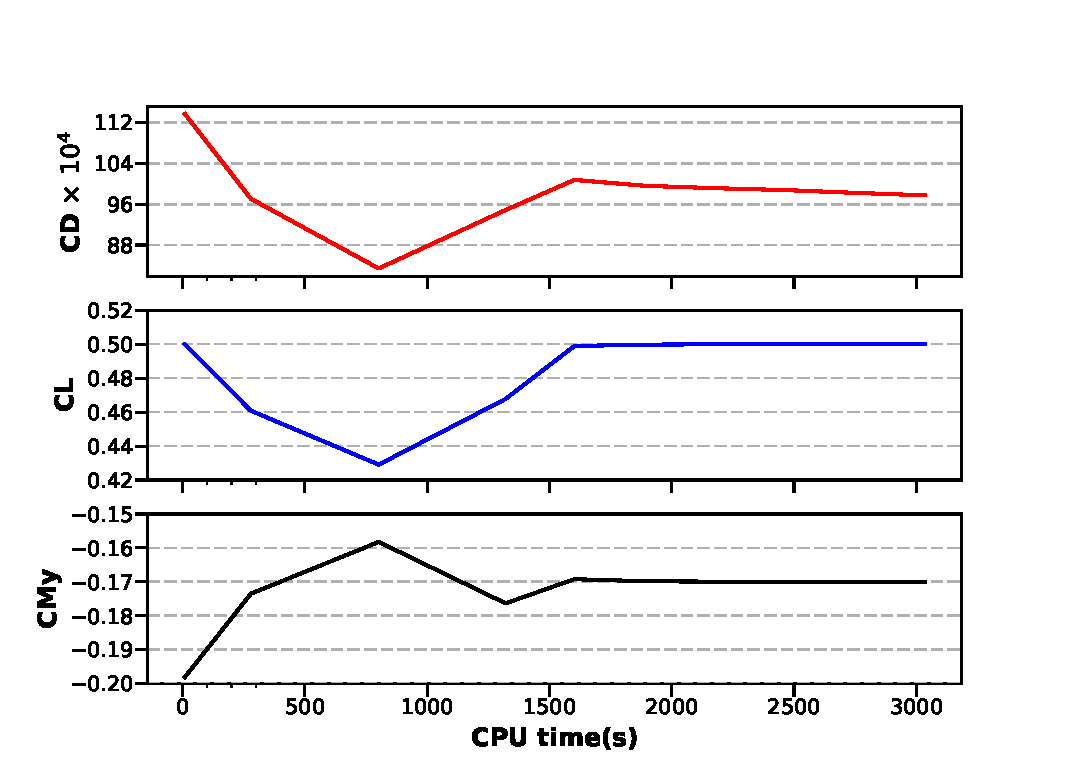
\includegraphics[clip,width=0.55\textwidth]{./figs/chap7_aso/kona/L1_480_cdlm.eps} }
  % \hspace{1em}
   \caption{Convergence histories for L1 grid, no. of design 480 \label{fig:kona_480}}
\end{figure}
\begin{figure}[H]
  \centering
   \subfloat[\label{fig:kona768opt}]{
   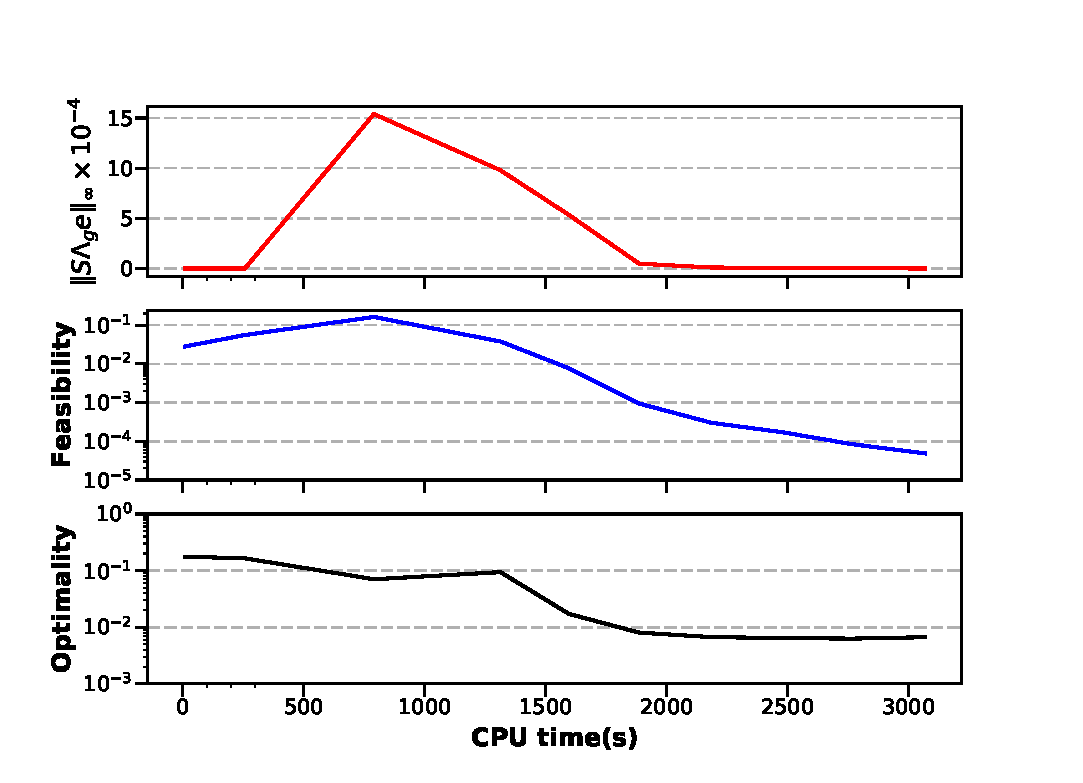
\includegraphics[clip,width=0.55\textwidth]{./figs/chap7_aso/kona/L1_768_comp_opt_feas.eps} }
  % \hspace{1em}
  \subfloat[\label{fig:kona768cd}]{
   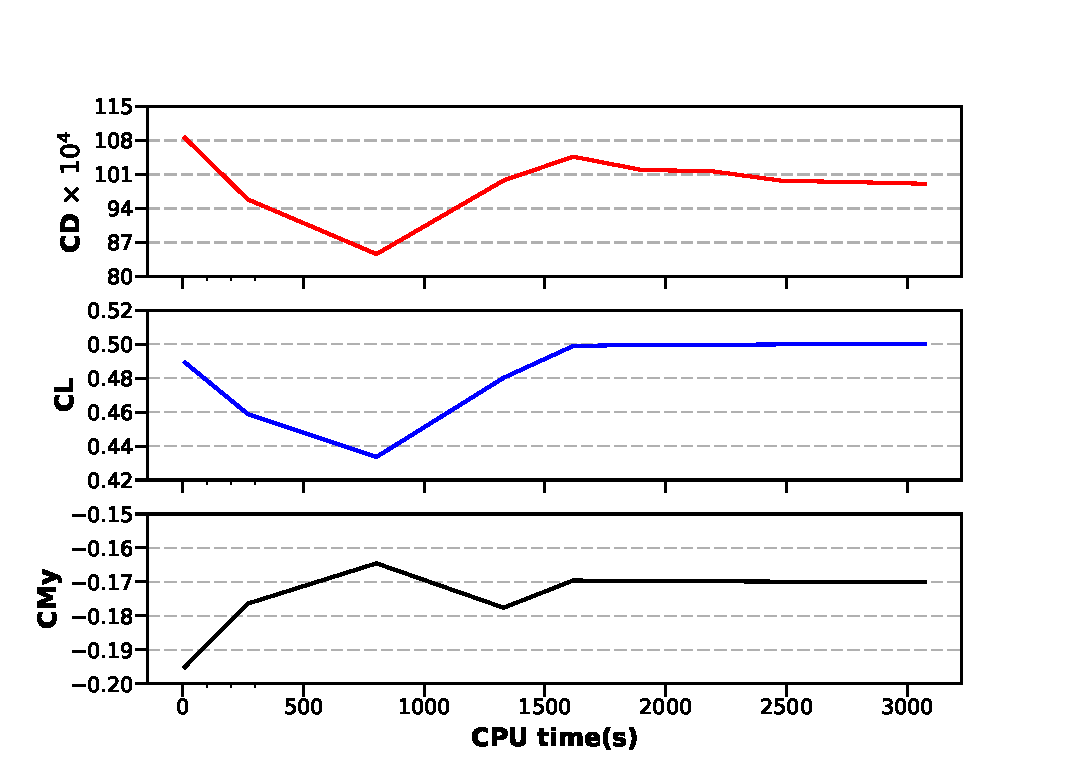
\includegraphics[clip,width=0.55\textwidth]{./figs/chap7_aso/kona/L1_768_cdlm.eps} }
%   \hspace{1em}
   \caption{Convergence histories for L1 grid, no. of design 768 \label{fig:kona_768}}
\end{figure}


\subsection{Results-SNOPT}
Figure~\ref{fig:sn_192}, \ref{fig:sn_480}, and \ref{fig:sn_768} shows the plots for the L1 grid, with no. of 
design variables ranges from 192, 480 to 768 using SNOPT. 

\begin{figure}[H]
  \centering
   \subfloat[\label{fig:sn192opt}]{
   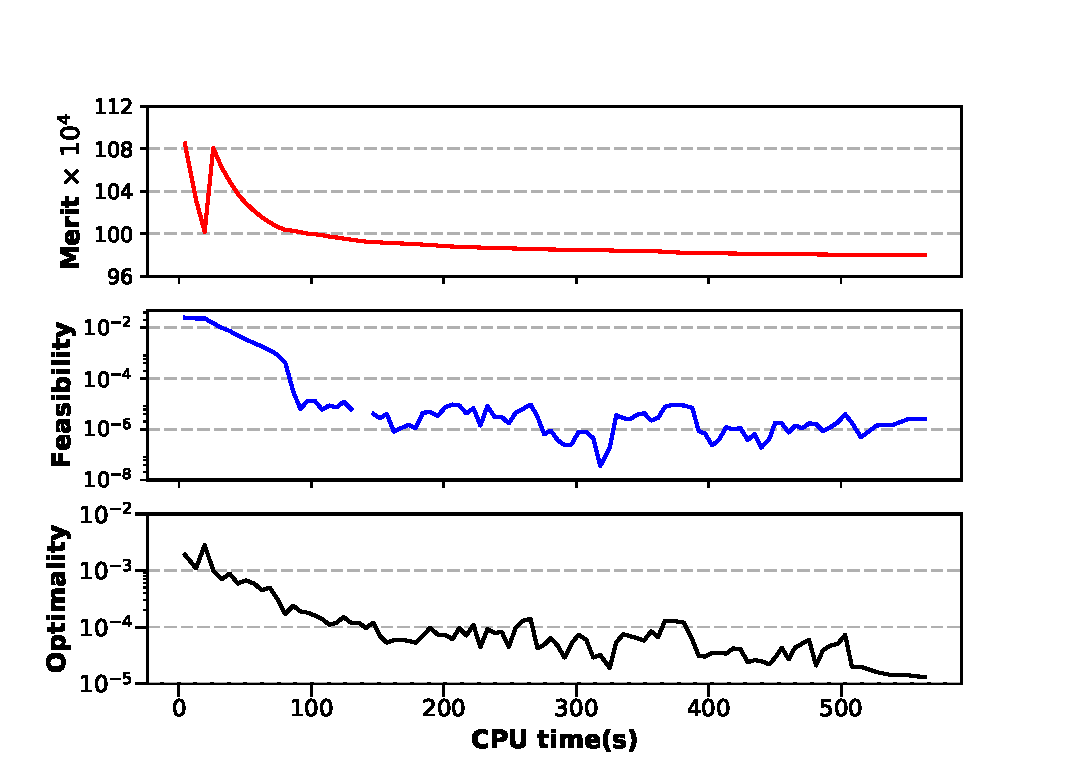
\includegraphics[clip,width=0.55\textwidth]{./figs/chap7_aso/snopt/L1_192_opt_feas.eps} }
  % \hspace{1em}
  \subfloat[\label{fig:sn192cd}]{
   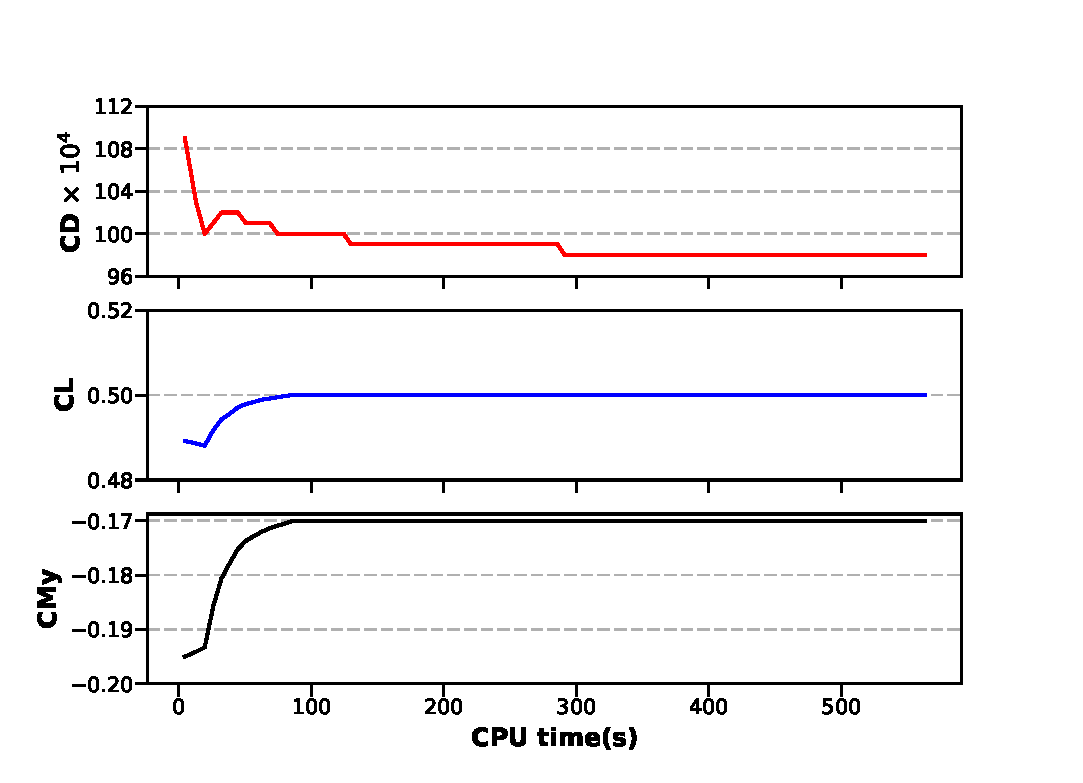
\includegraphics[clip,width=0.55\textwidth]{./figs/chap7_aso/snopt/L1_192_cdlm.eps} }
  % \hspace{1em}
   \caption{Convergence histories for L1 grid, no. of design 192 \label{fig:sn_192}}
\end{figure}

\begin{figure}[H]
  \centering
   \subfloat[\label{fig:sn480opt}]{
   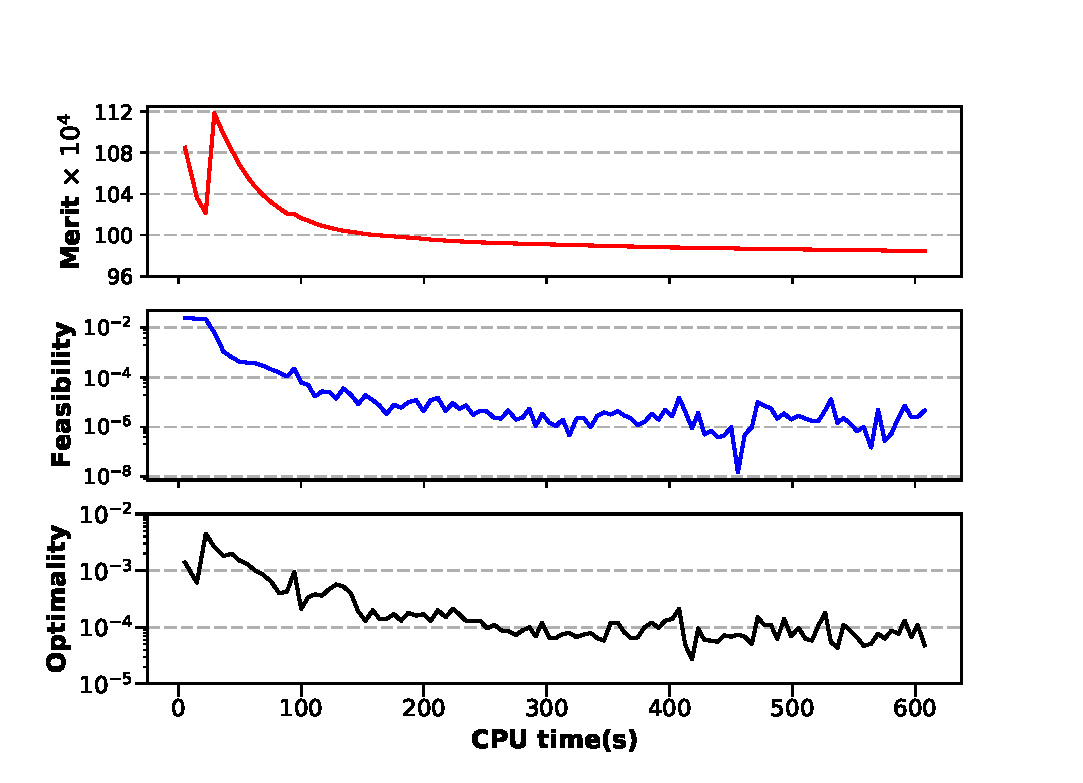
\includegraphics[clip,width=0.55\textwidth]{./figs/chap7_aso/snopt/L1_480_opt_feas.eps} }
  % \hspace{1em}
  \subfloat[\label{fig:sn480cd}]{
   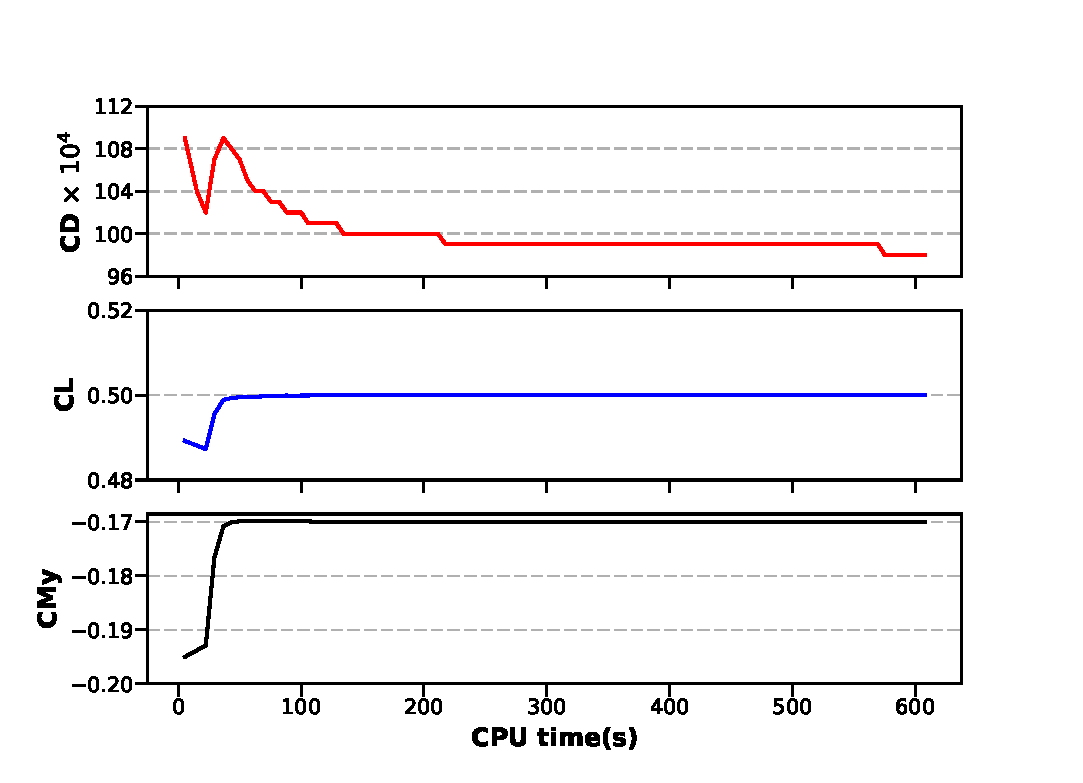
\includegraphics[clip,width=0.55\textwidth]{./figs/chap7_aso/snopt/L1_480_cdlm.eps} }
  % \hspace{1em}
   \caption{Convergence histories for L1 grid, no. of design 480 \label{fig:sn_480}}
\end{figure}
\begin{figure}[H]
  \centering
   \subfloat[\label{fig:sn768opt}]{
   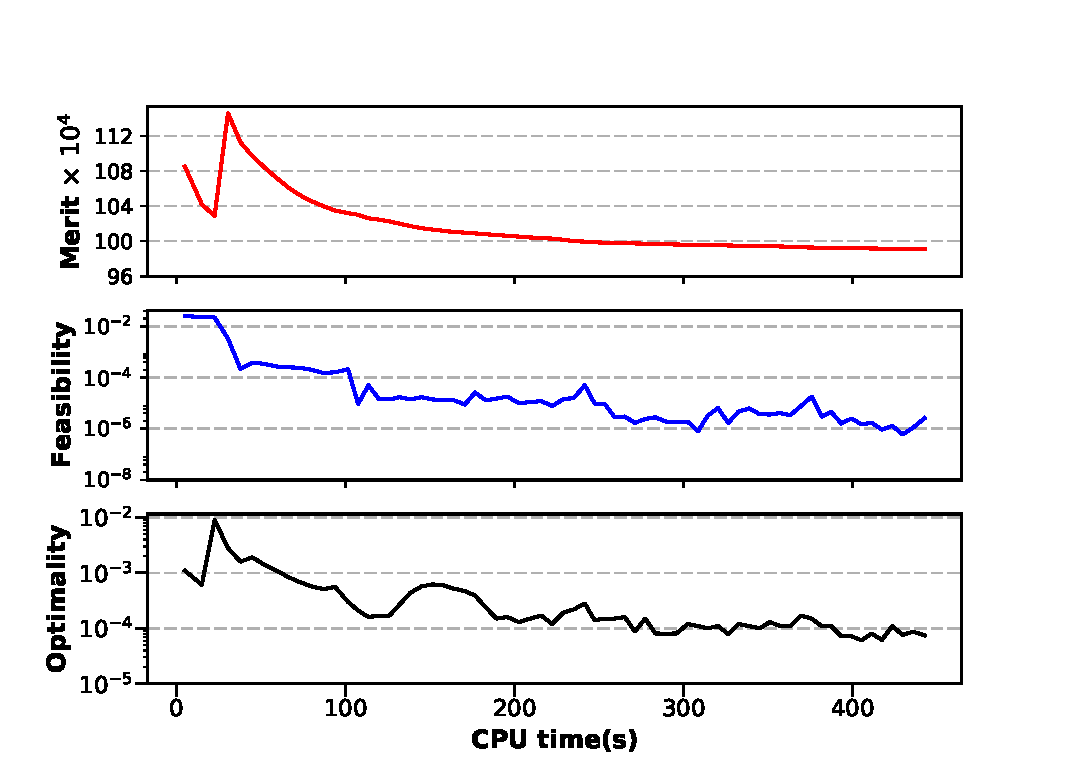
\includegraphics[clip,width=0.55\textwidth]{./figs/chap7_aso/snopt/L1_768_opt_feas.eps}}
  % \hspace{1em}
  \subfloat[\label{fig:sn768cd}]{
   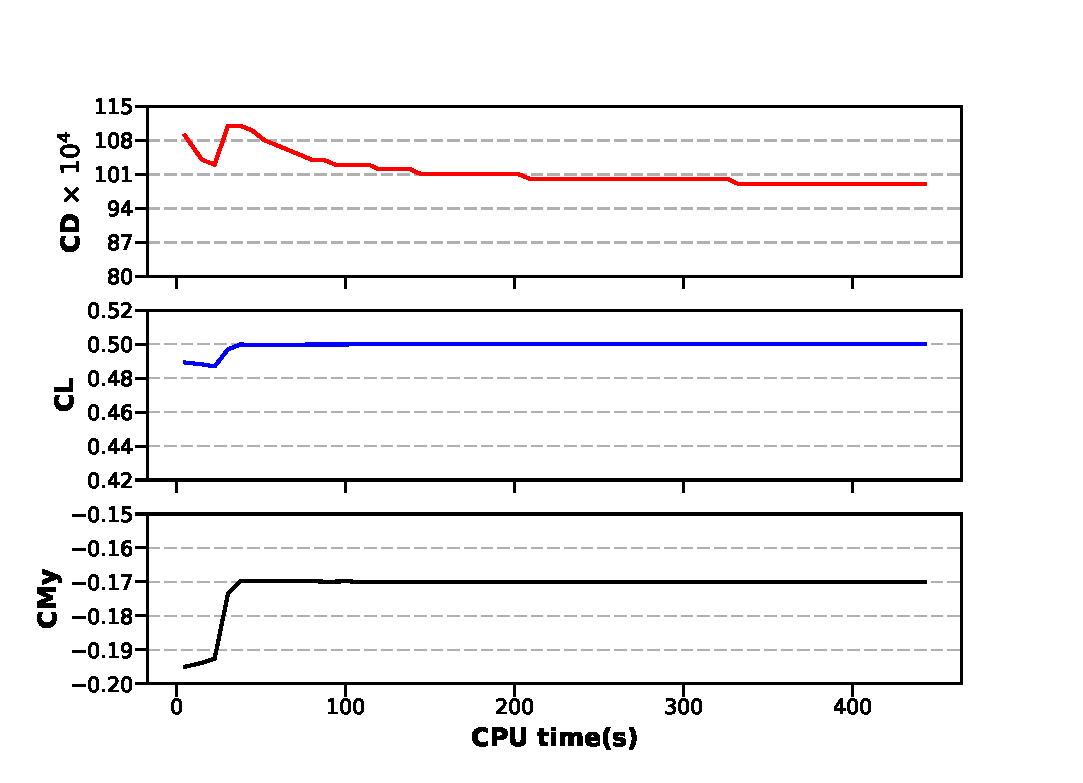
\includegraphics[clip,width=0.55\textwidth]{./figs/chap7_aso/snopt/L1_768_cdlm.eps} }
%   \hspace{1em}
   \caption{Convergence histories for L1 grid, no. of design 768 \label{fig:sn_768}}
\end{figure}

\subsection{Discussion}
The results above show that the Homotopy RSNK method can solve the Aerodynamic Shape Optimization 
problem in its original form based on Euler. However, its speed is much slower than SNOPT. Consequently, 
the scalability performance plot is not made. The low speed of Kona is largely due to the not so effective, but still 
better than not being used, preconditioner. Because the there are only two nonlinear aerodynamic constraints in this problem, $CL$ and $CMy$, while the rest of the inequality constraints are large amount of linear geometric constraints, $750$ thickness constraints, $1$ volume constraint, the preconditioner is lumping the nonlinear and linear inequality constraints together when making SVD approximations.  The parameters used in Kona is listed as follows: 

$\alpha_0=0.05,  \delta_{\text{targ}}=10, \phi^{\circ}_{\text{targ}}=20, n_{\mat{\Sigma}}=20 $ \\

Suggestions for the next steps for this problem are proposed in the next chapter. 

%As \cite{Lyu2013b} observed significant difference between Euler-optimized shapes and RANS-optimized shapes, with Euler-optimized shapes have a sharp pressure recovery near the trailing edge, which is disobeys with physical laws, as such flow would separate near the trailing edge. They emphasized that it is important to incorporate the viscous compressible effects in transonic wing shape design. 
%%%%%%%%%%%%%%%%%%%%%%%%%%%%%%%%%%%%

%%% Local Variables: 
%%% mode: latex
%%% TeX-master: t
%%% End: 
